\section{Влияние флуктуаций параметров экспонирования на результирующий профиль}

Разработанная модель СЭЛТР позволяет исследовать влияние параметров процесса на профиль линии, получаемой методом СЭЛТР.
В том числе эта модель может использоваться для исследования влияния флуктуаций параметров экспонирования на результирующий профиль линии.
Как и ранее, считалось, что экспонирование резиста в процессе СЭЛТР производится \linebreak ``в кадр'' с параметрами кадра, описанными в разделе~\ref{sec:verification}.
В качестве исходных параметров экспонирования были приняты $E$ = 20 кэВ, $T$ = 150~$^\circ$C, $t_\mathrm{exp}$ = 100 c и \linebreak $I$ = 4.56 нА, диаметр пучка составлял 600 нм, начальная толщина слоя ПММА -- 500 нм, зависимость температуры образца от времени при его охлаждении описывалась экспериментальной кривой охлаждения, приведенной на рисунке~\ref{fig:exp_cooling} (профиль линии, получаемой при этих параметрах процесса СЭЛТР, приведен на рисунке~\ref{fig:DEBER_4_profiles}a).
Поскольку в этом случае в резисте на момент остывания отсутствуют микрополости, среднеквадратичное отклонение точек промоделированных профилей было принято равным 2 нм (рисунок~\ref{fig:DEBER_sigmas}).
Далее определялись значения параметров экспонирования (энергии пучка, тока экспонирования и температуры образца), при которых отклонения точек промоделированного профиля от исходного были сопоставимы со среднеквадратичным отклонением при моделировании (рисунки~\ref{fig:DEBER_vary_E}, \ref{fig:DEBER_vary_I} и \ref{fig:DEBER_vary_T}).

\begin{figure}[h!]
	\begin{center}
		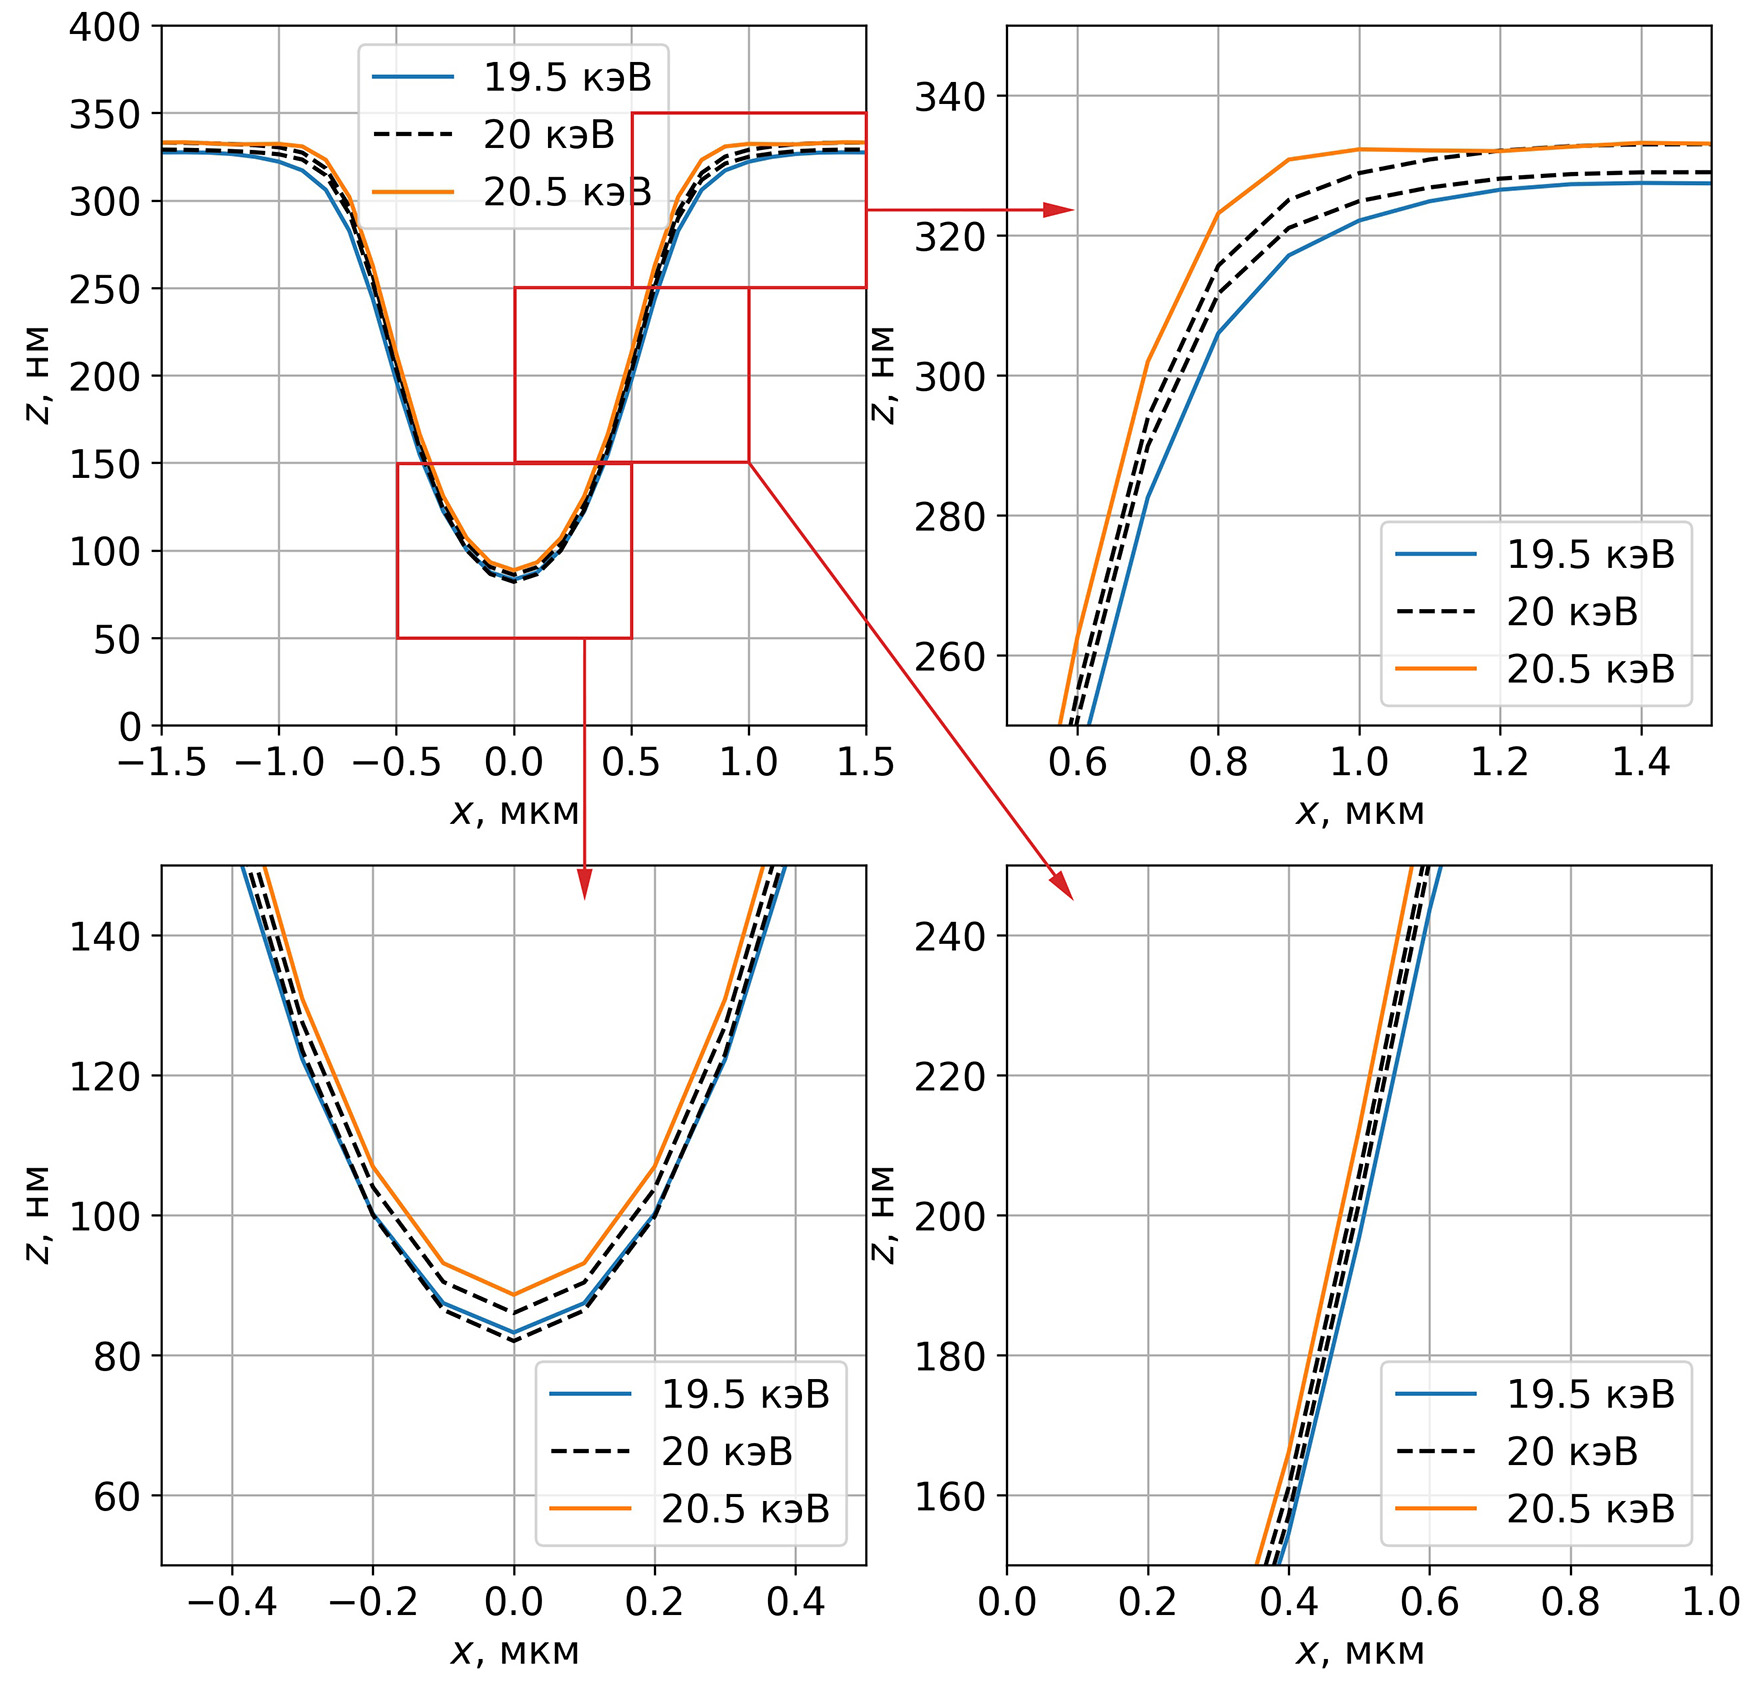
\includegraphics[width=\linewidth]{DEBER_stability/vary_E_4_arrows_200_CUT}
	\end{center}
%	\vspace{-1em}
	\caption{Изменения профиля линии, полученной методом СЭЛТР, вызванные отклонениями энергии пучка от исходного значения 20 кэВ при $T$~=~150~$^\circ$C, $t_\mathrm{exp}$ = 100 c и $I$ = 4.56 нА.}
%	\vspace{1em}
	\label{fig:DEBER_vary_E}
\end{figure}

\begin{figure}[h!]
	\begin{center}
		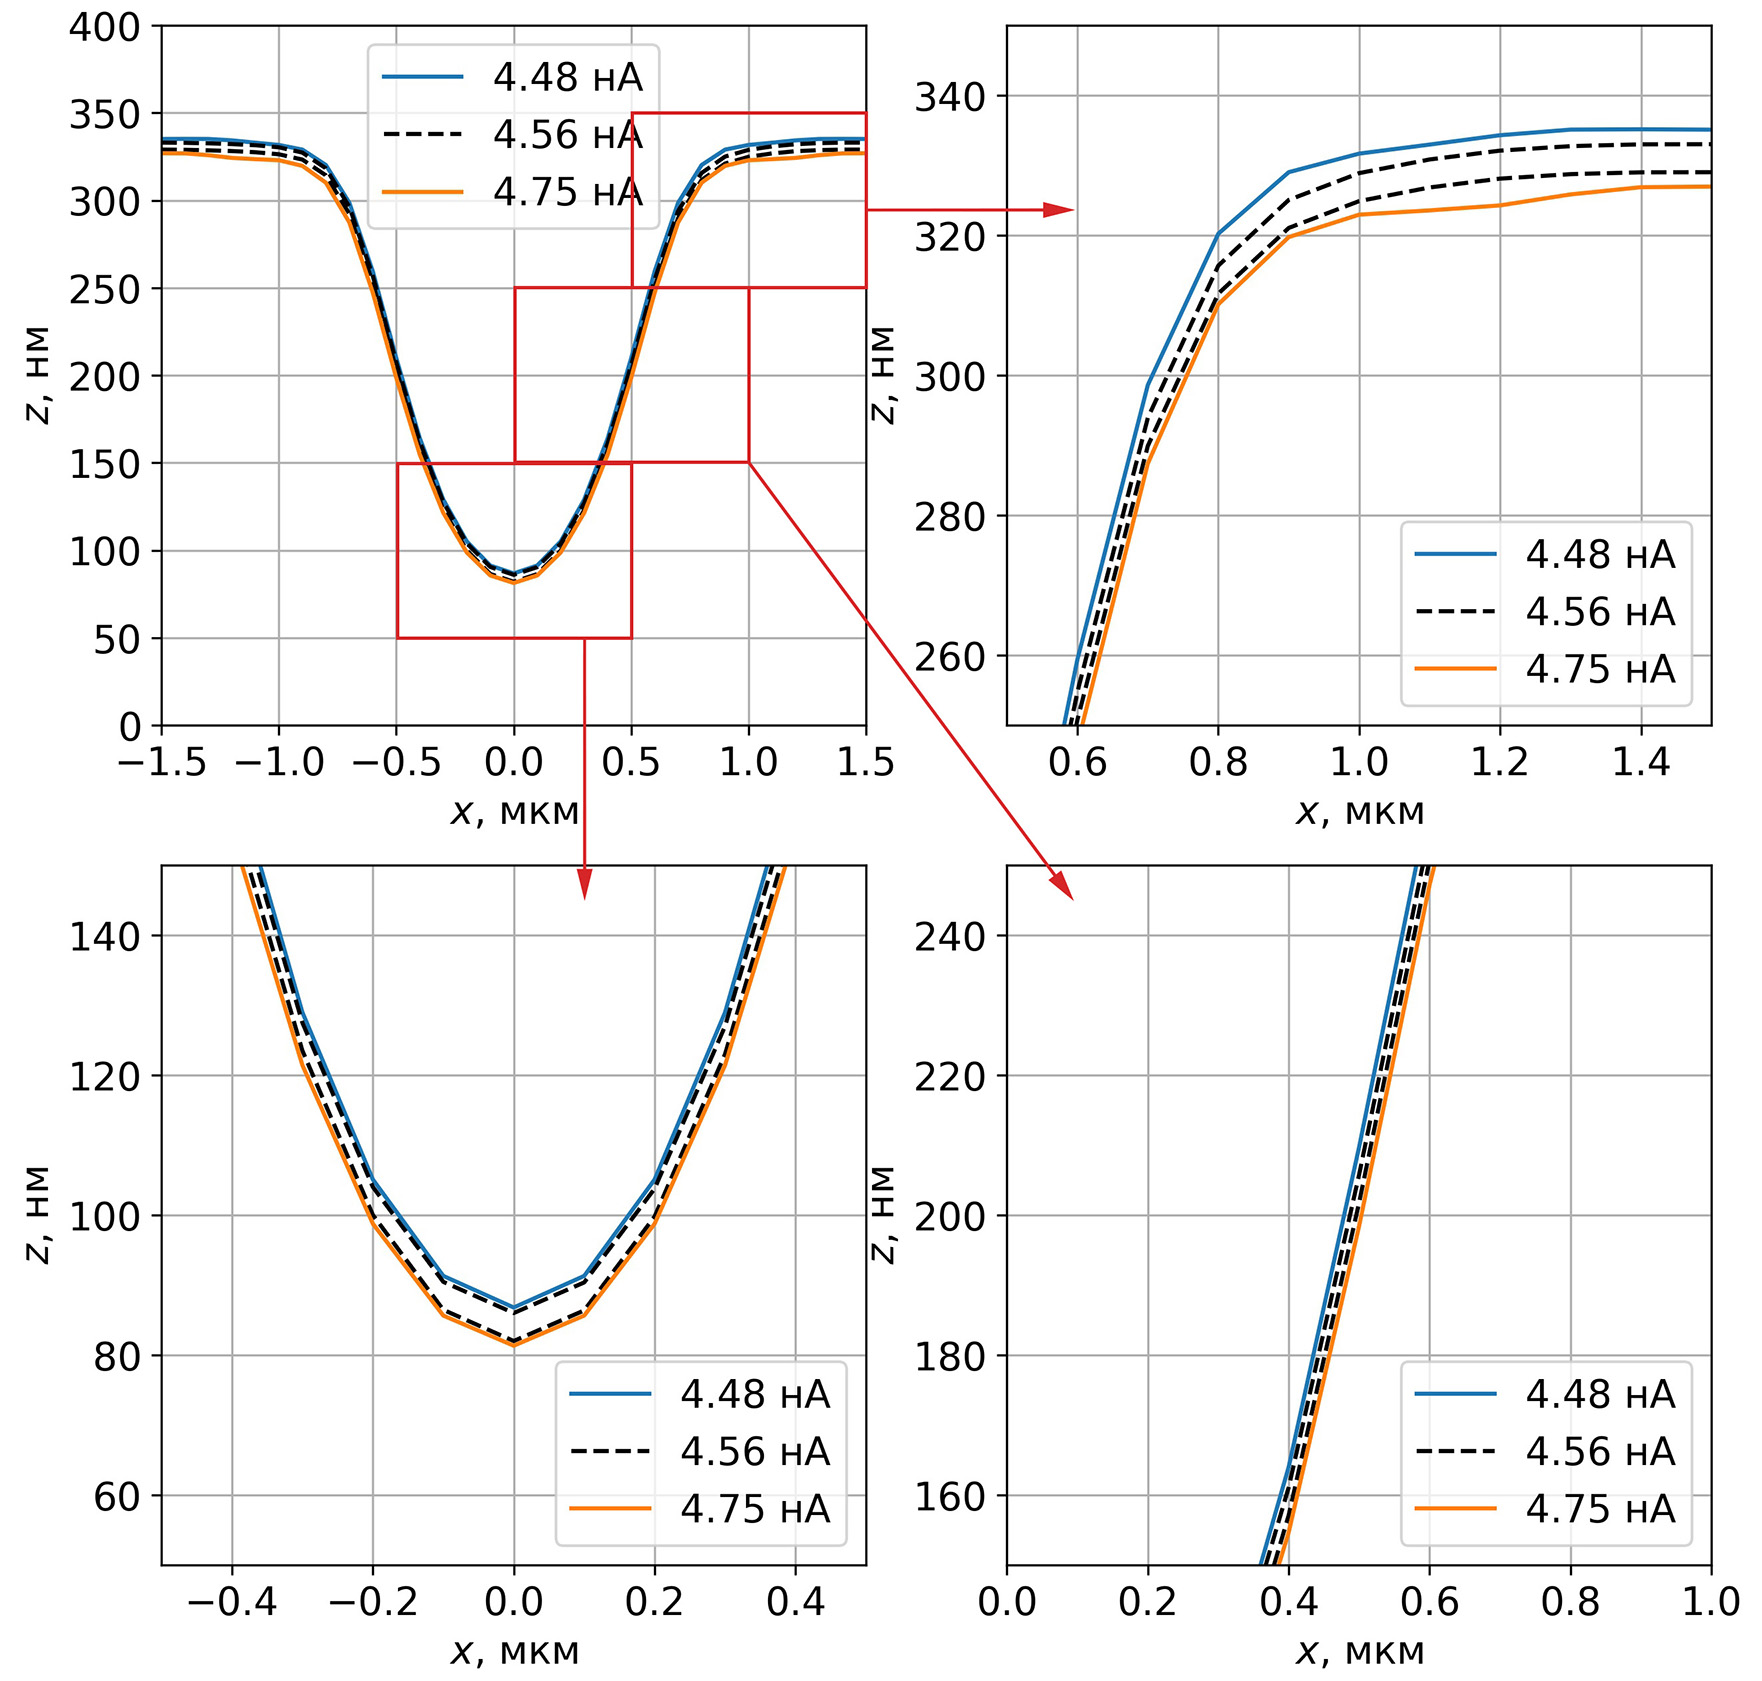
\includegraphics[width=\linewidth]{DEBER_stability/vary_I_4_arrows_200_CUT}
	\end{center}
%	\vspace{-1em}
	\caption{Изменения профиля линии, полученной методом СЭЛТР, вызванные отклонениями тока экспонирования от исходного значения 4.56 нА при $E$ = 20~кэВ, $T$ = 150~$^\circ$C и $t_\mathrm{exp}$ = 100 c.}
	\label{fig:DEBER_vary_I}
\end{figure}

\begin{figure}[h!]
	\begin{center}
		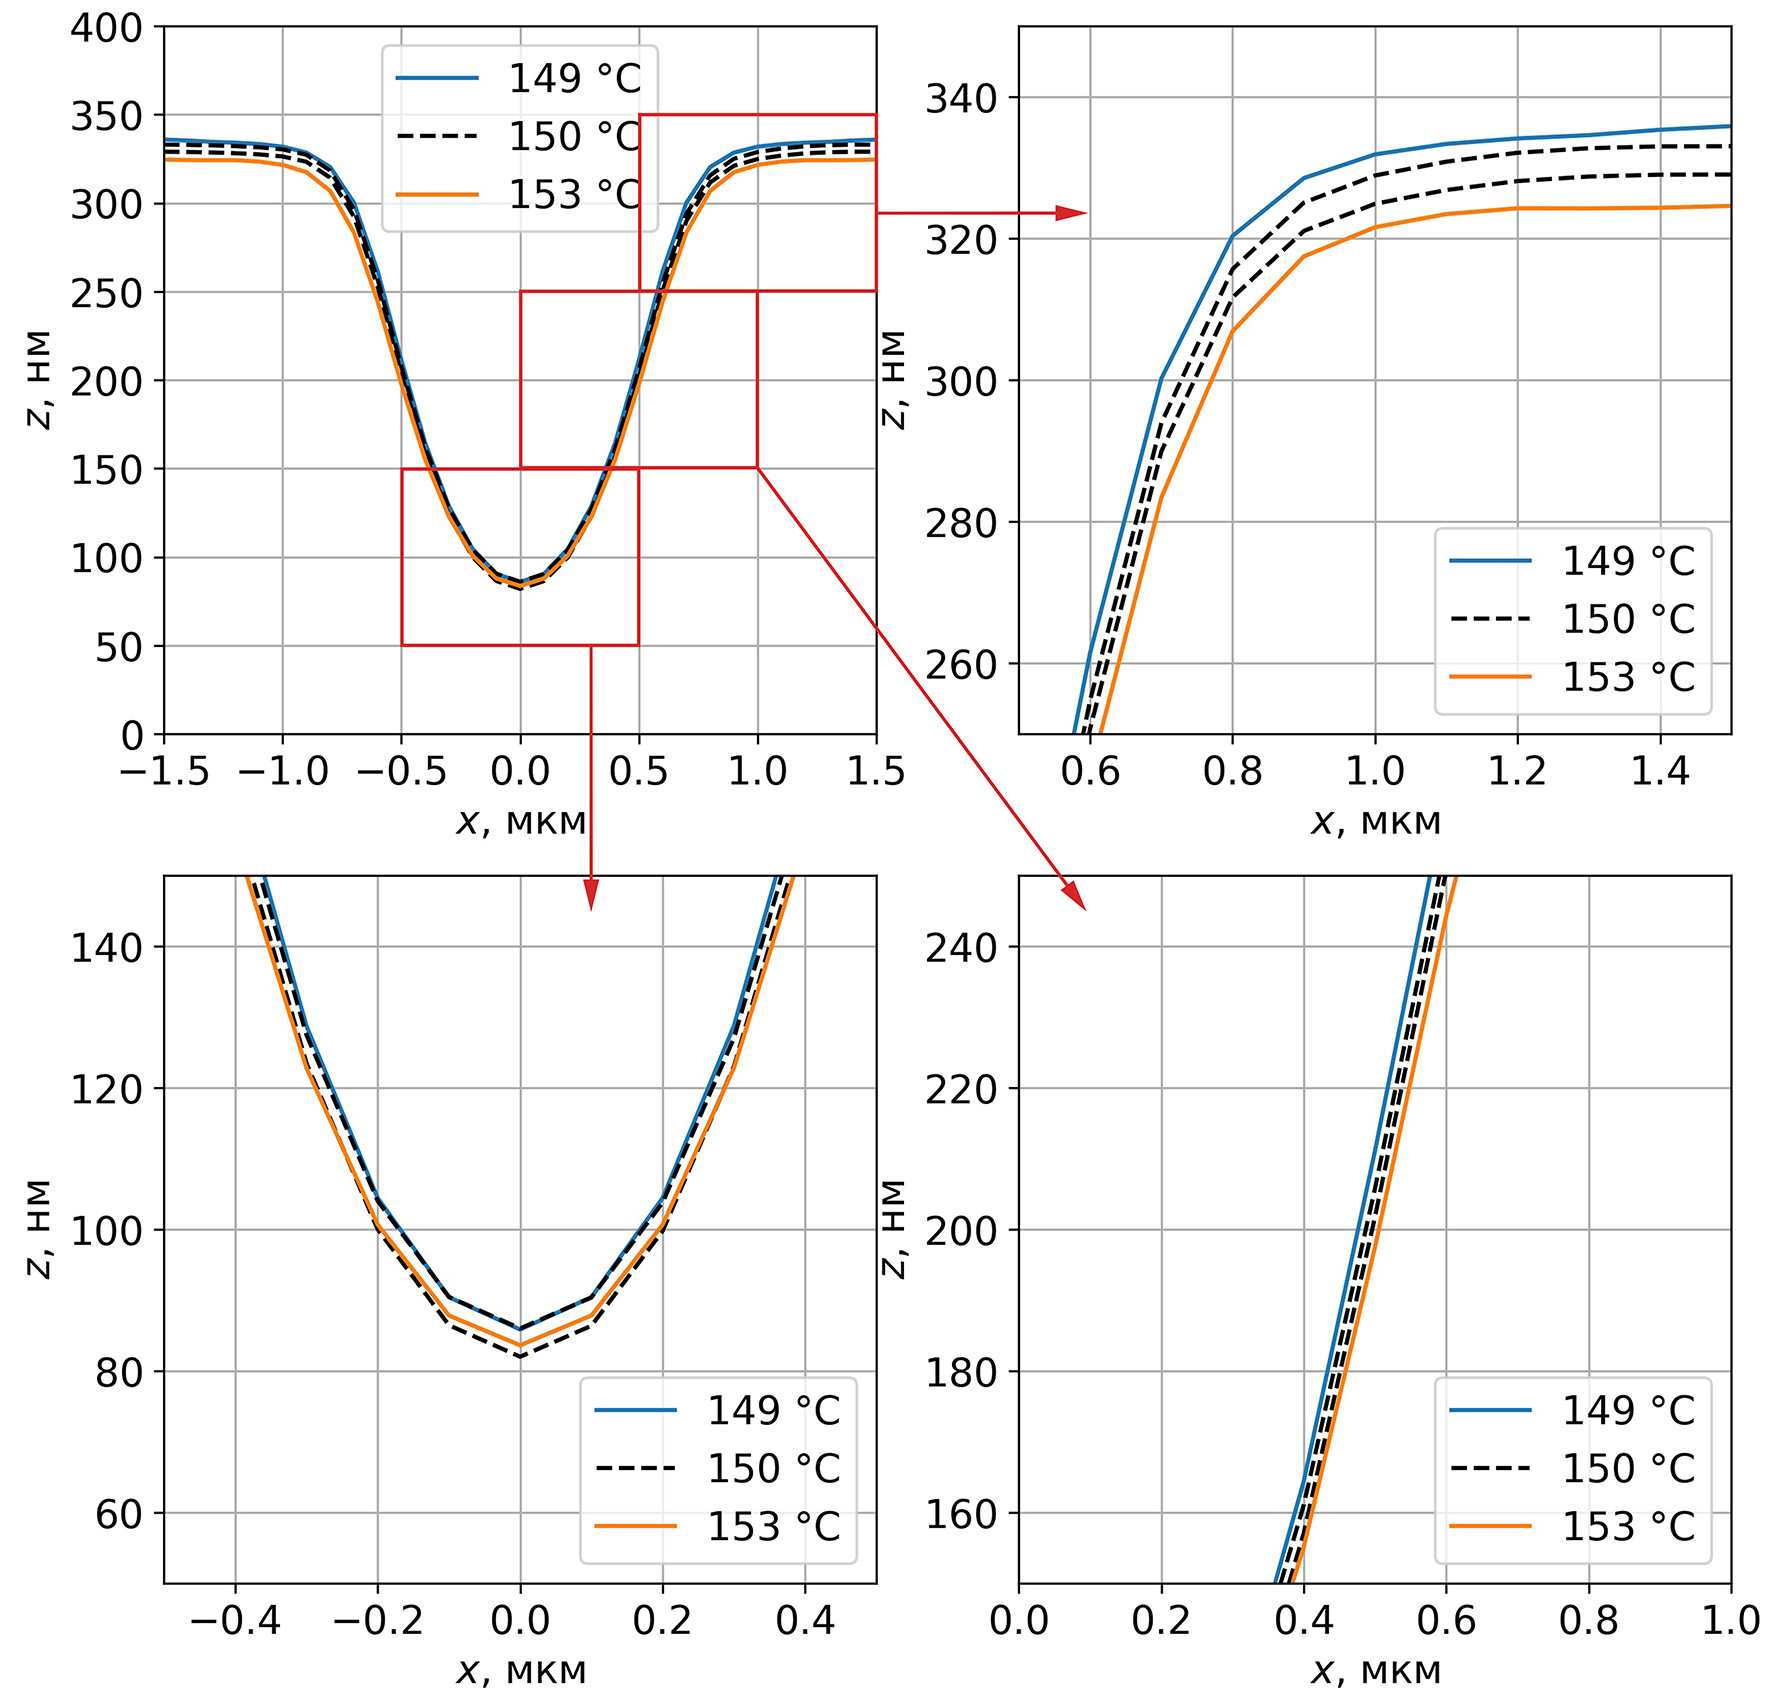
\includegraphics[width=\linewidth]{DEBER_stability/vary_T_4_arrows_200_CUT}
	\end{center}
	\vspace{-0.5em}
	\caption{Изменения профиля линии, полученной методом СЭЛТР, вызванные отклонениями температуры образца от исходного значения 150~$^\circ$C при $E$ =~20 кэВ, $t_\mathrm{exp}$ = 100 c и $I$ = 4.56 нА.}
	\label{fig:DEBER_vary_T}
	\vspace{0.5em}
\end{figure}

Как показано на рисунках~\ref{fig:DEBER_vary_E}, \ref{fig:DEBER_vary_I} и \ref{fig:DEBER_vary_T}, интервалы значений энергии пучка, тока экспонирования и температуры образца, при которых точки промоделированного профиля находятся в пределах 2 нм от исходного профиля, составляют примерно 19.5--20.5 кэВ, 4.48--5.75 нА и 149--153~$^\circ$C соответственно.
Таким образом, в качестве требований к стабильности параметров экспонирования в методе СЭЛТР могут быть приняты максимально допустимые значения флуктуаций энергии пучка, тока экспонирования и температуры образца, составляющие 0.5~кэВ, 0.1~нА и 1~$^\circ$C соответственно.
